\chapter{Antecedentes}
\section{Estado del arte}
\subsection{Caracter�sticas de la memoria}

Tama�o de cluster que impone fat32 \cite{fat32_1} \cite{fat32_2}

\subsection{Descripci�n de equipos}
Para poder realizar los experimentos hemos contado con dos equipos en el laboratorio. Son dos equipos con procesador AMD Phenom (tm) X6 1055T, con 7'6 GiB de RAM. En los que hemos instalado Debian 6.0.6, que viene con el kernel 2.6.32-5-amd64.

Ambos dos forman parte de una red interna de \url{gf.tel.uva.es}, teniendo cada uno de ellos los siguientes hostnames:
\begin{itemize}
\item Leonardo, con la IP: 192.168.0.50.
\item Donatello, con la IP: 192.168.0.51.
\end{itemize}

Como esta red no est� accesible desde el exterior de la escuela, para poder trabajar desde casa y tener monitorizado los experimentos, hemos recurrido a los tuneles ssh y al commando screen de Linux, que detallamo en la siguiente secci�n \ref{subsec:ComoTrabajarDesdeFueraETSiT}.

\section{Utilidades}

\subsection{Comandos y herramientas utilizadas}
\subsubsection{Comando Linux}
En Linux existen mulitud de comandos que nos han facilitado el trabajo a la hora de realizar este Proyecto. Uno de los m�s importantes ha sido \verb|dd|.
\begin{itemize}
\item \verb|dd|: \textit{Copia un fichero, convirtiendo y formateando seg�n los operandos}.
En principio este comando se usa para crear copias de un disco, en nuestro caso creamos archivos \verb|.iso| de las memorias USB. Pero en unas pruebas nos dimos cuenta de que ten�a mayor rendimiento que el comando \verb|cp|, que es el originario de Linux para copiar ficheros, y desde ese momento lo hemos usado tambi�n para la copia ``normal''. Por defecto sus bloques de copiado son de 1024bytes y sus par�metros son los siguientes:
\begin{verbatim}
$ dd if=ruta_o_fichero_entrada of=fichero_salida
\end{verbatim}
\item \verb|df|: \textit{Uso del espacio del sistema de ficheros}.
Este comando te da informaci�n sobre el espacio de los dispositivos montados en el sistema. A parte de ver el espacio disponible en las memorias, principalmente se ha utilizado para ver la capacidad que ten�an las memorias y comprobar si su capacidad se ha visto recudida, ver /ref{experiementoFlash}. Nota importante:
\begin{verbatim}
$ df --block-size=kB \\ Muestra un tama�o de bloque de 1000bytes
$ df --block-size=k \\ Muestra un tama�o de bloque de 1024bytes
\end{verbatim}
\item \verb|hexdump|: \textit{Muestra el contenido de un fichero en ascii, decimal, hexadecimal, u octal}.
Gracias a la orden:
\begin{verbatim}
$ hexdump -c .iso > .txt
\end{verbatim}
Podemos crear un archivo de texto con el que luego comprar con \verb|meld|, de esta manera podemos comparar im�genes \verb|iso| de forma muy f�cil y ver sus diferencias.
\item \verb|iotop|: \textit{Muestra el proceso de las peticiones de lectura o escritura que implican a distintos dispositivos del sistema}.
Gracias a este comando podemos monitorizar si una lectura o escrita a la memoria sigue en curso o murio su proceso.
\item \verb=ls -l | wc -l=: Esta orden muestra la cantidad de elementos en un directorio, ha sido de mucha utilidad sobre todo en el experimento de /ref{tabladenombres}.
\item \verb|od -x .txt|: \textit{Muestra un fichero en octal y otros formatos}.
Hemos utilizado ficheros en hexadecimal, como ficheros base de lectura y escritura en este proyecto, este comando ha ayudado a visualizar esos ficheros hexadecimales.
\end{itemize}
\cite{manLinux}
\cite{Programaci�ndeShellScripts}

\subsubsection{Bash y Shell script}
Bash es ...

Gracias a estos Shell script hemos podido automatizar procesos que podr�an llevar muchos d�as y filtar los resultados para una mejor comprensi�n de los mismos.

\subsubsection{Control de versiones y Git}
Git es una herramienta para el control de versiones. Tiene muchas virtudes, pero la m�s importante para este caso es poder tener un historio de cada cambio ``comiteado'', lo que nos permite tener una copia de seguridad casi perfecta tanto del c�digo como de la redacci�n de Proyecto. En cualquier momento podemos volver a un punto anterior o ver que se cambiado de un fichero en concreto \cite{git-scm}. Todo el Proyecto se ha ido guardando en \url{github.com}, que permite crear repositorios git de manera gratuita siempre que estos sean de libre acceso, en esta direcci�n del mismo: \url{https://github.com/jilgue/flashcrash}.

\subsection{�Com� trabajar desde fuera de la ETSiT?}
\label{subsec:ComoTrabajarDesdeFueraETSiT}
Se puede tardar d�as en conseguir resultados, para monitorizar el proceso es necesario conectarse a los equipos y poder recuperar la shell donde tenemos lanzado el script. Para ellos nos hemos ayudado del protocolo SSH y el comando screen.

\subsubsection{SSH}
SSH es un protocolo de shell remota segura. Gracias a ello podemos conectarnos al terminal de un ordenador y ejecutar ordenes en �l.

SSH usa una autenticaci�n con cable publico/privada. Si queremos conectarnos por ssh sin tener que escribir la contrase�a cada vez, tenemos que generar una pareja de claves y a�adir la publica a nuestro servidor:
\begin{verbatim}
$ ssh-keygen -t rsa -b 2048
\end{verbatim}

Esto nos genera un \verb|.pub| dentro de la carpeta \verb|.ssh| y tenemos que copiar su contenido en el archivo \verb|.ssh/authorized_keys| del servidor. Con esto la pr�xima vez que nos conectemos no tendremos que escribir la contrase�a \cite{Criptograf�aasim�trica}.

\subsubsection{Tunelando con ssh}
En la escuela tenemos una arquitectura parecida a esta \ref{fig:Esquemadered}:

\begin{figure}
	\centering
		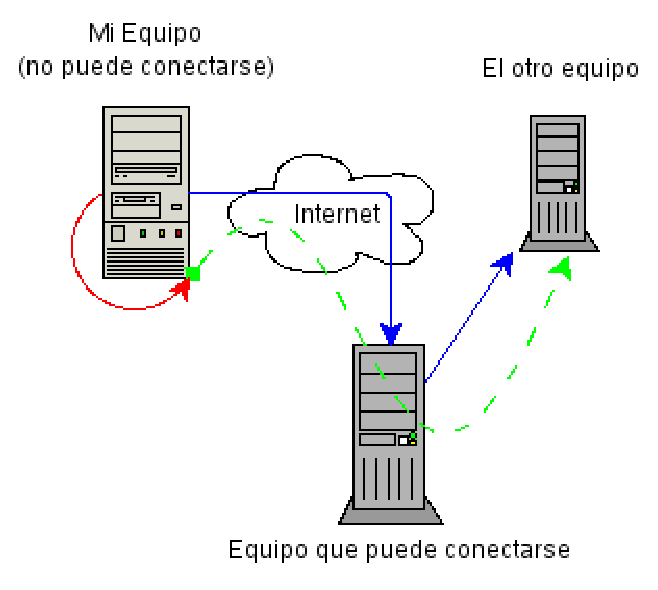
\includegraphics[width=0.60\textwidth,natwidth=299,natheight=266]{fig/tunel-ssh2}
	\caption{\emph{Esquema de red}}
        \label{fig:Esquemadered}
\end{figure}

Desde ``Mi equipo'' no puedo conectarme al ``Otro equipo''. Para solvertar este problema creamos un tunel:
\begin{verbatim}
$ ssh -L 2222:donatello:22 -L 2221:leonardo:22 usuario@gf.tel.uva.es
\end{verbatim}

Con esta linea hemos abierto un t�nel desde nuestro puerto 2222 y 2221 al 22 de donatello y leonardo respectivamente a trav�s de \url{gf.tel.uva.es}. Ahora para conectarnos a nuestro t�nel escribimos en nuestro terminal:
\begin{verbatim}
$ ssh usuario@localhost -p2221 -X
$ ssh usuario@localhost -p2222 -X
\end{verbatim}

\subsubsection{Screen}
Screen es una herramienta que nos permite recuperar una sesi�n shell. Podemos dejar corriendo un script cerrar la conexi�n, irnos a casa, abrir una conexi�n nueva y recuperar la misma terminal que ten�amos antes.

Uso b�sico de \verb|screen|:
\begin{verbatim}
$ screen // abre una sesi�n
Ctrl + a + d // deja la sesi�n en background.
$ screen -r // recupera la sesi�n
\end{verbatim}
\cite{Usodet�nelessshyscreen}
\cite{Usob�sicodescreenenLinux}
